\documentclass{article}

\usepackage[final]{neurips_2019}
\usepackage{array,multirow,graphicx}

\usepackage[utf8]{inputenc}
\usepackage[T1]{fontenc}
\usepackage{hyperref}
\usepackage{url}
\usepackage{booktabs}
\usepackage{amsfonts}
\usepackage{nicefrac}
\usepackage{microtype}
\usepackage{graphicx}
\usepackage{xcolor}
\usepackage{lipsum}
\usepackage{enumitem}
\usepackage{amsmath}
\usepackage{float}
\usepackage{multicol}
\usepackage{pgfplots}
\usepackage{subcaption}


% \setlength{\parskip}{0pt}
% \setlength{\parsep}{0pt}
% \setlength{\headsep}{0pt}
% \setlength{\topskip}{0pt}
% \setlength{\topmargin}{0pt}
% \setlength{\topsep}{0pt}
% \setlength{\partopsep}{0pt}

% \linespread{0.95}

% \usepackage[compact]{titlesec}
% \titlespacing{\section}{0pt}{*0}{*0}
% \titlespacing{\subsection}{0pt}{*0}{*0}
% \titlespacing{\subsubsection}{0pt}{*0}{*0}

\newcommand{\note}[1]{\textcolor{blue}{{#1}}}

\title{
  Generative Pre-Training Language Models \\
  with Auxiliary Conditional Summaries\\
  \vspace{0.3em}
  \small{\normalfont Stanford CS224N Custom Project Final Report\\
  \textbf{Mentor:} Amaury Sabran; We choose to have our project graded (Option 3)}  % Select one and delete the other
}

\author{
  Yutong (Kelly) He \\
  Stanford University \\
  \texttt{kellyyhe@stanford.edu} \\
  % Examples of more authors
  \And
  Junshen Kevin Chen \\
  Stanford University\\
  \texttt{jkc1@stanford.edu}
  \And
  Phillip Kim \\
  Stanford University \\
  \texttt{pkkim@stanford.edu}
}

\begin{document}

\maketitle

\vspace{-1em}

% \begin{multicols*}{2}

%%%%%%%%%%%%%%%%%%%%%%%%%%%%%%%%%%%%%%%%%%%%%%%%%%%%%%%%%%%%%%%%%%%%%%%%%%%%%%%%%%%%%%%%%%%%%%%%%%%%%%%%%%%%%%%%%%%%%%%%% ABSTRACT

\begin{abstract}
% \textit{An abstract should concisely (less than 300 words) motivate the
% problem, describe your aims, describe your contribution, and highlight your
% main finding(s).}

The goal for this project is enhance the GPT-2\cite{gpt2} model's conditional synthetic text generation ability and resolve the issue of GPT-2 model persistent bias with human guidance. With an auxiliary input of a human-written text as the intended summary of the generated text, we aim to generate text that is on topic, consistent and fluent. We approach this problem by first encoding the summary with BERT\cite{bert}, and then use the encoded state in conjunction with GPT-2 to produce an on-topic next token probability distribution with three different novel model structures: BERT-GPT LMH, BERT-GPT DAU and BERGPT.

We use a dataset of CNN news articles with their respective summary text to train and evaluate our models with two experiment settings and four metrics. We find that while all models achieve decent results, the original GPT-2 models still remains the best records for most of the experiments. We have also discovered three quantitative evaluation metrics that are semantically meaningful and agree with human qualitative evaluation.
\end{abstract}

%%%%%%%%%%%%%%%%%%%%%%%%%%%%%%%%%%%%%%%%%%%%%%%%%%%%%%%%%%%%%%%%%%%%%%%%%%%%%%%%%%%%%%%%%%%%%%%%%%%%%%%%%%%%%%%%%%%%%%%%% INTRO


\section{Introduction }

% \textit{The introduction explains the problem, why it’s difficult, interesting, or important, how and why current methods succeed/fail at the problem, and explains the key ideas of your approach and results. Though an introduction covers similar material as an abstract, the introduction gives more space for motivation, detail, references to existing work, and to capture the reader’s interest.}

The GPT-2 model, a transformer decoder trained over a large corpus of English text, is able to generate text very convincingly, as if it is written by a human. This generation starts with a optionally user-defined text "prompt", then performs next-word generation conditioned by all previous text including the prompt itself and any generated token. However, there is no control mechanism to ensure that the generated text stays on the topic intended by the user, and GPT models are known to be prone to bias and incorrect statement in generated text\cite{github}. BERT, on the other hand, is a powerful encoder that transforms any given text a language representation, and can be fine-tuned to perform various tasks. Experiments have shown that BERT is able to achieve state-of-the-art sentence-level language understanding with its bidirectional training strategy\cite{bert}.

In this project, we aim at solving the problem that can be considered as an inverted text summerization task. With an input initial segment and an input summary, the model should output a piece of text that is coherent with both the initial segment and the input summary, as well as maintaining grammatical correctness. We leverage BERT's ability to encode information in text, and use this encoding as a method to control the text generation process of GPT-2, thus solving the problem of "text generation conditioned on topic". On a high level, we adopt a pre-trained BERT model to encode the summary text of a given article, inject this information into GPT at different parts of the model, and train language models with the target article. We develop three different models: \textbf{BERT-GPT LMH}, \textbf{BERT-GPT DAU} and \textbf{BERGPT} to tackle this problem.

Using these approaches, we find that although all models are able to generate human-interpretable synthetic text for the majority of the time, the original GPT-2 model still achieves the best performance in 6 out of 10 quantitative metrics and all human evaluation metrics we adopt. We also discover that the quantitative metrics we choose are consistent with the human qualitative evaluation results. We consider such discovery as part of our contribution in this project that these quantitative metrics can be used in future study on similar topics.


%%%%%%%%%%%%%%%%%%%%%%%%%%%%%%%%%%%%%%%%%%%%%%%%%%%%%%%%%%%%%%%%%%%%%%%%%%%%%%%%%%%%%%%%%%%%%%%%%%%%%%%%%%%%%%%%%%%%%%%%% RELATED WORK


\section{Related Work}

\subsection{Generative Pre-Training (GPT) Models}
While numerous unlabelled text corpus exists, labelled datasets for specific tasks are rare and small most of the time. Meanwhile, Transformer\cite{transformer} has shown to perform efficiently and effectively in learning long-term language structures and in obtaining a more robust transfer learning performance. Inspired by such discrepancy and Transformer, GPT\cite{gpt} and its successor GPT-2\cite{gpt2} were published in 2018 and 2019 respectively to investigate the ability of the transformer model to learn a universal representation that can transfer the natural language understanding knowledge acquired with unsupervised language modeling to a wide range of other tasks that require supervision with little adaptation.

Since the date of release, GPT models has drawn a lot of attention from the field. As mentioned earlier, OpenAI has published a follow-up model called GPT-2 which enhances the performance of the original GPT model. As the purpose of its design, GPT models have helped researchers achieve better language understanding models, and have developed better strategies in various directions such as long sequence generation\cite{sparsetransformer} and cross-lingual language modeling\cite{crosslingual}. GPT models have also been applied in fields of music to create coherent and realistic music pieces with different styles. Most significantly, the success of the GPT models has inspired researches focusing on the ability to transfer knowledge obtained with unsupervised language modeling. Many state-of-the-art models such as BERT\cite{bert}, Tranformer-XL\cite{transformerxl} and Xlnet\cite{xlnet} developed upon GPT models.

Though achieving state-of-the-art performance on 9 out of the 12 different natural language understanding tasks at the time of publication, GPT models have some limitations that have been widely discussed\cite{github} yet insufficiently investigated by researchers. We are particularly interested in the fact that even though Transformer models are known for long-term memory preservation, the GPT models is sometimes unable to generate contents consistent with the given prompt. Moreover, the generation of the GPT model is not controllable, that is, with the same input seed sentences, the model is likely to generate drastically different contents each experiment. Since the dataset on which the GPT models have trained on consists of some bias and factual inaccuracies, sometimes the GPT models also generates statements that are produces the same bias or inaccuracy similar to the training data. Last year, Salesforce released CTRL\cite{ctrl}, with which they experimented GPT-2 generation with controlled settings. CTRL, however, did not involve modifying the model structure of GPT-2, nor did it provide comprehensive quantitative evaluation metrics.

In our project, we are inspired to focus on the generative aspect of the model and resolve these issues with auxiliary summary input and corresponding architecture modifications, and provide semantically meaningful evaluation metrics for our experiments.

\subsection{BERT as an Encoder}

BERT \cite{bert} has proven to be a key advancement in Machine Learning and NLP by achieving state-of-the-art results in many NLP tasks, including question answering and natural language inference. By applying bi-directional training of the encoder part of Transformer \cite{transformer}, researchers have developed a new method called Masked LM (MLM), allowing for training on un-annotated text drawn from the web. Results of the model show that bidirectional training is much more effective at building a better understanding of language context and flow than single-direction language models.

On top of being a well-performing language representation model, BERT is versatile in that it is able to be quickly fine-tuned for a variety of NLP tasks. In order to fine-tune BERT for a specific task, only one additional layer is necessary for the pre-trained BERT model as opposed to substantial architectural modifications. Use of transfer learning has become a norm for state-of-the-art research using BERT. For example, BERT has inspired the making of RoBERTa \cite{liu2019roberta}, a replication study of BERT where modified hyperparameters and longer training led to better results, and XLNet \cite{xlnet}, a generalized auto-regressive pretraining method.

BERT's versatility and ease of use underscores the cooperative nature of our objective. By using BERT to encode texts, we aim to take advantage of BERT's powerful understanding of language to be able to achieve better control over the text generation process of GPT-2.


%%%%%%%%%%%%%%%%%%%%%%%%%%%%%%%%%%%%%%%%%%%%%%%%%%%%%%%%%%%%%%%%%%%%%%%%%%%%%%%%%%%%%%%%%%%%%%%%%%%%%%%%%%%%%%%%%%%%%%%%%  APPROACH



\section{Approach}

In this project, we attempt the following task: with an input summary, design models that output a piece of text that is coherent with the input summary, as well as maintaining grammatical correctness and fluency.

The training objective for all models is to maximize:
\begin{align}
    \mathcal{L}(\mathcal{D}) = \sum_{(x,y)} \log P(x^m|x^1, x^2, ..., x^{m-1}, y^1, y^2, ..., y^n; \Theta)
    \label{lm_objective}
\end{align}
where $\mathcal{D}$ is the dataset consisting of articles represented as $x$ paired with their summaries represented as $y$. $x^i$ is the $i$-th token in the article and $y^j$ is the $j$-th token in the summary, assuming the article has $m$ tokens and the summary has $n$ tokens. $P$ is the probability distribution of the next token in the generated sentences given all the previous tokens and the auxiliary summary. $\Theta$ is the parameters defined by our model architectures.

The same training objective can also be expressed as
\begin{align}
    \mathcal{L}(\mathcal{D}) = \sum_{(x,y)} \log P_y(x^m|x^1, x^2, ..., x^{m-1}; \Theta)
    \label{conditional_objective}
\end{align}
where $P_y$ represents the language model probability distribution parameterized by the auxiliary summary $y$.

While equation \ref{lm_objective} depicts the goal of the problem as a special case of the traditional language modeling, equation \ref{conditional_objective} shows that we can also encode the summary and use it as ones of the parameters of the language modeling. Based on the different expressions of the training objectives, we propose three different approaches: \textbf{BERT-assisted GPT Language Model Head}, \textbf{BERT-assisted GPT Distribution Adjustment} and \textbf{BERGPT} to solve the conditional language modeling problem and compare them with the original GPT-2 model.

\subsection{Baselines: Vanilla GPT-2}

We use an unmodified version of GPT-2, as the baseline to be compared to. The original GPT-2 model already satisfies the training objective defined in Equation \ref{lm_objective}. We experiment this model with two different settings described as the following.

\paragraph{Unconditioned text generation:}
To use as a comparison to completely unconditioned generated text, we use the GPT model only the end-of-sentence token as input prompt and sample to generate text (of random topic), without any fine-tuning. We include this setting of GPT-2 to examine the natural behavior of its generation.

\paragraph{Topic as prompt:}
A naive way to condition the generated text on topic is to use the summary text itself as the prompt to the GPT model. We expect the generated text to be generally similar to texts on the same topic, but deviate in content from the summary. This setting can be considered as the equivalence of the CTRL model\cite{ctrl} as we use the summary text as the control code for generation. We use this model as a baseline to evaluate our other approaches against it.

\subsection{BERT-GPT LMH: BERT-assisted GPT Language Model Head}

We introduce our first method: BERT-assisted GPT Language Model Head model (BERT-GPT LMH): GPT takes a context text, encodes it with an embedding unit, forward it through a transformer unit, then forward the transformer output encoding through a language model head, to get an output vector of logits, which is finally used to sampled the next word. 

In this approach, we intervene the GPT language model by keeping the original model up to the transformer unit, discarding the old language model head, and re-training a language model head, with its input augmented by an encoding of the summary text as BERT outputs. We take the BERT encoding vectors, max-pool / average-pool it along the word axis, then concatenate it with the GPT transformer output. The resultant encoding is a vector of size $n_{BERT} + n_{GPT}$ where $n_{BERT}$ represents the dimension of the last hidden layer of BERT, which is equivalent to the BERT embedding dimension for a single token, and $n_{GPT}$ represents the dimension of the last hidden layer of GPT, which is equivalent to the GPT embedding dimension. In practice, both $n_{BERT}$ and $n_{GPT}$ are equal to 768. This is then inputted into a fully-connected layer (i.e. a new language model head) with output size equal to the vocabulary size $V$, thus completing the language model. 

We train this language model by freezing all of BERT and GPT up to the transformer unit, and optimize only parameters of the fully connected layer.

\begin{figure}[h]
    \centering
    \begin{subfigure}[t]{0.5\textwidth}
        \centering
        \includegraphics[scale=0.25]{bert_lm.png}
        \caption{Re-trained language model head with BERT and GPT}
    \end{subfigure}%
    ~ 
    \begin{subfigure}[t]{0.5\textwidth}
        \centering
        \includegraphics[scale=0.25]{bert_gpt_adj.png}
        \caption{Adjusting output distribution with BERT encoding}
    \end{subfigure}
    \caption{Model structures of BERT-GPT LM (left) and BERT-GPT DA (right)}
\end{figure}

\subsection{BERT-GPT DAU: BERT-assisted GPT Distribution Adjustment Unit}

Similar to the approach above, intuitively, we may adjust the next word distribution by biasing it towards on-topic words. In this approach, we keep both BERT and GPT unchanged, taking the output encoding of BERT, max-pool / average-pool on along the word axis, then feed it into a feed forward unit, such that the input of the fully-connected layer is the size of the last hidden layer of BERT $n_{BERT}$ and its output is the vocabulary size $V$. 

Since $n_{BERT} = n_{GPT} = 768$, we can then take this output vector and add it to the output of GPT, thus adjusting the distribution of the next word. We optimize only parameters of the FC layer immediately after BERT pooling, while freezing the GPT and BERT in their entirety.

We attempt to add attention to the summary text in each layer in GPT. We achieve this by similarly encoding the text with BERT as before, then adding a multi-head attention unit immediately before GPT's feed-forward output. This is equivalent to a complete transformer constructed by BERT as its encoder and GPT as its decoder. However, given the timeline of this project, we will only add the additional attention in the later layers of the GPT model and train it by freezing BERT and all layers within GPT preceding the added units.


\subsection{BERGPT: A Transformer Built with BERT and GPT}

We propose BERGPT, a way to combine BERT and GPT while preserving its transformer structure intact \cite{transformer}. We use BERT as the encoder and GPT as the decoder for the conditional text generation task. This problem setup and network structure is analogous to a machine translation problem, where we aim to translate the summary text into an expanded article using this encoder-decoder structure.

With a target article $x$ with its paired summary $y$, the model first encodes the summary $y$ with the pre-trained BERT encoder and obtains $y_{enc} = BERT(y)$. Then, for each attention block in the original GPT model, on top of the self-attention layer and the layer normalization and fully-connected layer associated with it, we add another encoder-decoder attention block. The encoder-decoder attention block has a similar structure to the self-attention block: a multi-head attention block concatenated with a fully-connected layer, along with layer normalization and residual connections between the layers. The multi-head attention block, illustrated in Figure \ref{multi-head}, calculates the scaled dot-product attention of linearly projected vectors defined as query, key and value and outputs the linearly projected concatenation of the attention. The scaled dot-product attention is defined as the following:

\begin{align}
    Attention(Q,K,V) = softmax(\frac{QK^T}{\sqrt{d_k}})V
\end{align}

where $Q,K,V$ represent query, key and value respectively. $d_k$ is dimensionality of the query, key and value vectors.

However, instead of using the embedded article $x_{enc}$ as its query, key and value, the encoder-decoder attention block takes $y_{enc}$ as its key and value and $x_{enc}$ as its query and compute the corresponding scaled dot-product attention. As a result, the encoder-decoder attention is calculated as

\begin{align}
   Attention(x_{enc},y_{enc},y_{enc}) = softmax(\frac{x_{enc}y_{enc}^T}{\sqrt{d_k}})y_{enc}
\end{align}


\begin{figure}[h]
    \centering
    \begin{subfigure}[t]{0.5\textwidth}
        \centering
        \includegraphics[scale=0.55]{bergpt.png}
        \caption{Adding attention to BERT encoding (pink denotes added units and connections to GPT)}
    \end{subfigure}%
    ~ 
    \begin{subfigure}[t]{0.5\textwidth}
        \centering
        \includegraphics[scale=0.55]{multi-head attention.png}
        \caption{Multi-head Attention layer structure}
        \label{multi-head}
    \end{subfigure}
    \caption{Model structure of BERGPT. Here we show a simplified version where the encoder and decoder only have one BERT-encoder block and one GPT-decoder block respectively. In our experiments we follow the structure of the original BERT and GPT-2 model and have 12 layers of blocks for both the encoder and the decoder.}
\end{figure}

Same as the self-attention block, the encoder-decoder attention block also maps the input embeddings to output vectors with the same dimensionalities. As a result, the encoder-decoder attention block serve as a portable component to the entire model structure. In our experiment, we connect the encoder-decoder attention block only to the last layer of the self-attention block in the original GPT model. In practice, one can add the encoder-decoder attention block to any layers of the self-attention block in the GPT model. 

Due to computation limitation, we were not able to train or fine-tune all the parameters in the BERGPT model. Therefore, we only train and fine-tune the parameters that are downstream to the additional encoder-decoder attention blocks and keep the other parameters frozen. Moreover, for the same reason, the final fully-connected layer, which serves as a language model head in our model, does not share weights with the input embedding matrix. In other word, in our experiment setting, we keep the original input embedding and learn a new language model head with the fully-connected layer. Nevertheless, if one is able to train and fine-tune the entire network, parameter sharing between the input embedding matrix and the language model head is more ideal.



%%%%%%%%%%%%%%%%%%%%%%%%%%%%%%%%%%%%%%%%%%%%%%%%%%%%%%%%%%%%%%%%%%%%%%%%%%%%%%%%%%%%%%%%%%%%%%%%%%%%%%%%%%%%%%%%%%%%%%%%%  EXPERIMENTS



\section{Experiments}

\subsection{Data}

We use a dataset of news articles extracted from The DeepMind Q\&A Dataset\cite{cnndailymail}, which is a large collection of news articles, and we focus on the CNN articles because each of these articles come with human-written highlights as reference summaries for each news article. There are a total of 92,580 highlight-story pairs.

We pre-process the data set by using Byte Pair Encoding (BPE)\cite{bpe}, as used in GPT-2. For each story, we separate the highlights from the articles so that we have our reference articles and summaries for separate model inputs. In our experiments, we preclude the articles that are shorter than 128 tokens and create separated training, development and testing set with ratio 90:5:5 which results in 82182 highlight-story pair for training, 4541 for development and 4595 for testing.

We use the highlights as the auxiliary conditional summaries and the stories as the target article to perform the on topic synthetic text generation task defined above. The inputs to our models are highlight text encoded by BERT, and target article text encoded by BPE tokenizer. The output of our models is the probability distribution of the next word, as a vector with size $V$, the vocabulary size.

\subsection{Experimental Details}

We train all our models with the AdamW optimizer\cite{adamw}, applying weight decay at $\lambda = 0.05$ during the process. We perform mini-batch gradient descent, and for the purpose of vectorization, each target article text is randomly sliced from the original piece with context length of 128 tokens. All models are trained with the maximum number of 30 epochs.

As described in the previous section, for all BERT-assisted GPT models, we freeze all the pre-trained parameters and only learn the additional parameters that connect the encoder and decoder. For BERGPT, we only add the encoder-decoder attention block to the last self-attention block of the decoder, which implies that we freeze all the pre-trained parameters in both BERT and GPT, and only train the encoder-decoder attention block and the new fully-connected layer serving as the language model head.

\subsection{Evaluation Metrics}

We adopt three quantitative evaluation metric and one human qualitative evaluation metric in our experiments.
\paragraph{Perplexity} 
We use perplexity to examine how well the models predict the target article samples. It is defined as the exponential of the cross entropy of the generated texts and the target texts. For the experiments, we report the average perplexities of all article-summary pairs.

\paragraph{ROUGE Scores}
We also use ROUGE scores \cite{lin-2004-rouge}, specifically the F1-score to evaluate the similarity between two texts. While this is often used as a metric of evaluation for text summarization models, it is equally applicable for our text expansion model by comparing our resultant generated article and reference article.

\paragraph{LDA + JSD} 
We use Latent Dirichlet Allocation \cite{NIPS2001_2070} to map all the generated articles to topic probability distributions that best capture all the words in the articles. We will then use Jensen–Shannon divergence to measure the similarity between the topic of the generated text and that of the target articles.

\paragraph{Human evaluation}
Besides the above quantitative evaluations, we ask human volunteers to assess fluency and topic cohesion of randomly chosen generated texts. Each assessor read 3 sets of generated articles, each set containing 6 articles generated by different models and the reference article with the same summaries, and decide the level of fluency and topic cohesion in the scale of 1 to 5, with 5 being the most fluent/coherent level.


\subsection{Results}

\subsubsection{Quantitative Metrics}
As presented in Table 1, our baseline model, the vanilla GPT-2 performs the best in almost all metrics with or without prompt. The notation "avg" and "max" here indicate the pooling strategy used for obtaining the BERT encoding of the summaries.  

In terms of perplexity, GPT-2 is a close second to BERT GPT DAU avg from performing the best for both with and without prompt experiments. On the other hand, BERGPT and BERT-GPT LMH max both have poor perplexity scores.

In terms of ROUGE scores, for the with prompt experiment, no models came close to the ROUGE scores of the vanilla GPT-2, but for the without prompt experiment, the ROUGE scores of the vanilla GPT-2 are closely tied for best with BERT-GPT LMH avg's scores.

The only category in which the vanilla GPT-2 does not come close to performing the best is the LDA + JSD metric for without prompt, where GPT-2 performs the worst. For this category, BERGPT performs the best without prompt and the worst with prompt, while all other models perform around the same level.

Overall, these results show that despite our modifications, the vanilla GPT-2 continues to perform the best in generating text in most categories.

\begin{table}[h]
    \centering
    \begin{tabular}{ |p{.2cm}|p{3.5cm}||p{1.6cm}|p{1.6cm}|p{1.6cm}|p{1.6cm}|p{1.6cm}| }
     \hline
     & \multicolumn{1}{c|}{Model} & \multicolumn{1}{c|}{Perplexity} & \multicolumn{1}{c|}{ROUGE-1} & \multicolumn{1}{c|}{ROUGE-2} & \multicolumn{1}{c|}{ROUGE-L} & \multicolumn{1}{c|}{LDA + JSD} \\
     \hline
     \parbox[t]{2mm}{\multirow{6}{*}{\rotatebox[origin=c]{90}{without prompt}}} & Vanilla GPT-2 & 22.603273 &  \textbf{0.16916494} & \textbf{0.01096475}& 0.12525628&  0.77531025 \\
     & BERT-GPT DAU avg & \textbf{21.910961} &  0.13497256& 0.00564681& 0.10807705  &  0.76744349 \\
     & BERT-GPT DAU max & 23.904585 &  0.13551144 & 0.00958346 & 0.11715993 &  0.74596844 \\
     & BERT-GPT LMH avg & 26.655932 & 0.15728040 & 0.00970389 &  \textbf{0.12619733}  &  0.75673676 \\
     & BERT-GPT LMH max & 29.783505 &  0.13424269 & 0.00868581 & 0.11138511   & 0.72097123  \\
     & BERGPT& 34.202326&  0.12938505 & 0.00893298 & 0.09586783   &  \textbf{0.68306939} \\
    %  & BERGPT init embed lr& &  0.06698157 & 0.00357837 & 0.05443442    & 0.71870444  \\
     \hline
     \parbox[t]{2mm}{\multirow{6}{*}{\rotatebox[origin=c]{90}{with prompt}}} & Vanilla GPT-2 & 17.822541 & \textbf{0.21963578}& \textbf{0.02569620}&  \textbf{0.17157309}   &  \textbf{0.56805357} \\
     & BERT-GPT DAU avg & \textbf{17.130703} & 0.14818597& 0.01777298& 0.13391426 &  0.57150789 \\
     & BERT-GPT DAU max & 18.780319 &  0.14683508& 0.01728999 & 0.13351382  &   0.57072197\\
     & BERT-GPT LMH avg & 21.409605 & 0.14820174 & 0.01676628 &  0.13103321 &  0.57946283 \\
     & BERT-GPT LMH max & 24.141396 &  0.14114764 &  0.01469263 & 0.12443054    &  0.57256593 \\
     & BERGPT& 30.709857&  0.13179502 & 0.00897114 & 0.09760922    & 0.65972524  \\
    %  & BERGPT init embed lr& &   0.07530547 &  0.00416835 & 0.06167900    & 0.68152079  \\
     \hline
    \end{tabular}
    
    \caption{Quantitative evaluation results. ROUGE-1 refers to the overlap of unigram between the target and generated articles, ROUGE-2 refers to the bigram overlap and ROUGE-L refers to the longest common subsequence based statistics.}
    \label{tab:my_label}
\end{table}


% \textbf{(Here we only need to describe the results, analysis can go to the next section. and dont worry abou the spacing too much i still need to write bergpt in the method section. Comment this one out after you read it :))}

% (wrong statement here, the bold ones are the best ones) yea, so doesnt GPT2 perform the best? close second for perplecity and rouge-L, i guess if you add "almost" before all lol

\subsubsection{Human evaluation results}

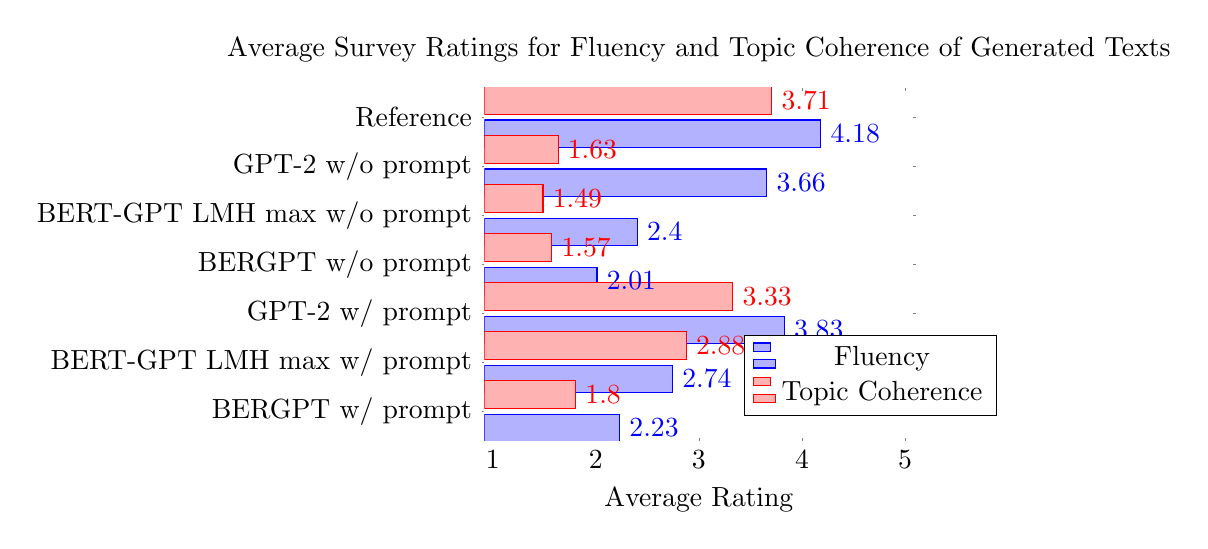
\begin{tikzpicture}
  \begin{axis}[title  = Average Survey Ratings for Fluency and Topic Coherence of Generated Texts,
    xbar,
    y axis line style = { opacity = 0 },
    xmin       = 1, xmax = 5,
    height=.5\textwidth,
    legend style={at={(0.9,0.07)},
                anchor=south,legend columns=1},
    tickwidth         = 1pt,
    ytick             = data,
    enlarge y limits  = 0.1,
    enlarge x limits  = 0.02,
    symbolic y coords = {BERGPT w/ prompt, BERT-GPT LMH max w/ prompt, GPT-2 w/ prompt, BERGPT w/o prompt, BERT-GPT LMH max w/o prompt, GPT-2 w/o prompt, Reference},
    nodes near coords,
    xlabel={Average Rating}
  ]
  \addplot coordinates { 
  (2.2317,BERGPT w/ prompt) (2.0122 ,BERGPT w/o prompt) (2.7439,BERT-GPT LMH max w/ prompt) (2.4024,BERT-GPT LMH max w/o prompt) (3.8293,GPT-2 w/ prompt) (3.6585,GPT-2 w/o prompt) (4.1829,Reference)} ;
  
    \addplot coordinates { 
  (1.8049,BERGPT w/ prompt) (1.5732,BERGPT w/o prompt) (2.8780,BERT-GPT LMH max w/ prompt) (1.4878,BERT-GPT LMH max w/o prompt) (3.3293,GPT-2 w/ prompt) (1.6341,GPT-2 w/o prompt) (3.7073,Reference)} ;
  
  \legend{Fluency, Topic Coherence}
  \end{axis}
\end{tikzpicture}

The survey results in the graph above show that the reference articles demonstrate the most fluency and topic coherence as expected. Besides the reference, we see that GPT-2 generated articles have the best fluency and topic coherence with or without prompt. We see that there is a wide discrepancy between the fluency of each model with or without prompt. With or without prompt, GPT-2 generated articles have significantly better ratings for fluency than the other two models. However, in terms of topic coherence, without prompt, each model performs at around the same level with low performance. On the other hand, with prompt, we see greater differences. GPT-2 performs the best, followed by BERT-GPT LMH max, followed by BERGPT. We can observe that the human evaluation results largely agree with the quantitative metrics we select in the previous section.


%%%%%%%%%%%%%%%%%%%%%%%%%%%%%%%%%%%%%%%%%%%%%%%%%%%%%%%%%%%%%%%%%%%%%%%%%%%%%%%%%%%%%%%%%%%%%%%%%%%%%%%%%%%%%%%%%%%%%%%%% ANALYSIS



\section{Analysis}

While we did not include the BERT-GPT DAU model in the human evaluation, we can observe that the perplexity results for other models are aligned with the human evaluation results of the fluency of the articles. From the perplexity metric alone, one may state that BERT-GPT DAU model performs the best, and is the only model that beats the vanilla GPT-2 both with and without prompt. However, qualitative results in the appendix indicate the model does not always yield human-level fluency. Observing examples (\ref{lm-wo}) (\ref{dau-wo}) (\ref{lm-w}) (\ref{dau-w}) from the appendix, we notice all the "bad" examples almost exclusively consist of multiple repeated sentences or phrases and the "good" examples for commonly consist of limited vocabulary and sentence structure.
One possible explanation is that the models overfit to the training data, which consists of only a few topics and similar writing styles, and therefore lacked the variation that comes with the vanilla GPT-2 model.
Perplexity does not always penalize repeated sentences or limited vocabulary heavily and therefore cannot guarantee a comprehensive evaluation on fluency. However, it does serve as a good indication of the model behavior.

Another noticeable factor in the perplexity and fluency evaluation result is that BERGPT achieves significantly lower perplexity and fluency evaluation results than all other models. When we look into the qualitative examples, we realize that the model still generates random tokens sometimes as shown in (\ref{bergpt-wo}) and ((\ref{bergpt-w})). The random generation does not only damage the fluency result, but also drastically diminishes the topic cohesion evaluation results of the model. As a result, we can also observe low scores in both quantitative and human evaluation topic cohesion results for BERGPT, even when we see high topic cohesion when the model does not generate random tokens. As a result, if we can resolve the issue of randomly generated tokens in BERGPT, it is possible to further improve its performance in all metrics. To do so, we can either increase the maximum number of epochs to prevent the model from underfitting, or train and fine-tune more or ideally all parameters to learn a better feature representation and potentially sharing the embeddings between the input embedding matrix and the final language model head.

From the human evaluation results, we also observe that BERT-GPT LMH model also performs poorly on topic coherence when used without a prompt, lower than the vanilla GPT-2 model, but is able to yield a high topic coherence when used with the highlight text as the generation prompt. We can study the cause of this by comparing the "good" examples of (\ref{lm-wo}) and (\ref{lm-w}) and observe that the generated text in (\ref{lm-w}) is a continuation of its highlight whereas the generated text in (\ref{lm-wo}) is about a similar but unrelated topic of its highlight. This difference shows that the re-trained language model is able to direct the generated passage towards a general topic of text, but is unable to stick to the correct details, whereas when used in conjunction with a highlight text prompt, not only is the model able to generate text coherent to the broad topic, but is able to stick to the correct details. BERT-GPT DAU model shows a similar behavior in its generated text. We may make the preliminary conclusion that the BERT-assisted GPT models are able to learn a general topic, but lack the refinement to generate specific texts. 



%%%%%%%%%%%%%%%%%%%%%%%%%%%%%%%%%%%%%%%%%%%%%%%%%%%%%%%%%%%%%%%%%%%%%%%%%%%%%%%%%%%%%%%%%%%%%%%%%%%%%%%%%%%%%%%%%%%%%%%%% CONCLUSION



\section{Conclusion}

In completing this project, we aimed to develop a model, such that when given an auxiliary input of humanly written text as the intended summary, the model would be able to generate a passage that is on topic, consistent, and fluent. To achieve this goal, we have attempted to modify GPT-2 to improve upon its ability to generate humanly convincing text consistent with its prompt, developing three different novel model structures: BERT-GPT LMH, BERT-GPT DAU and BERGPT. Using a dataset of CNN news articles with their respective summary text to train and evaluate our models, we found that while all models achieved decent results, the original GPT-2 model still performs the best in most experiments. However, in evaluating these models, we discovered that our human qualitative evaluations were largely representative of the quantitative evaluations ran on the models. In collecting these results, we have discovered three quantitative evaluation metrics, perplexity, ROUGE, and LDA + JSD, that are semantically meaningful and agree with human qualitative evaluation. Moving forward, we hope that these evaluation metrics will be able to be of use for similar text generation tasks in the future. Moreover, we plan to improve our models with further training and parameter learning strategies and we hope that our model can eventually make an impact on the problem we defined in this project.


\clearpage
\bibliographystyle{unsrt}
\bibliography{references}

% \end{multicols*}

\clearpage

\appendix

\section{Generated Samples: without Context Prompt}

In this section, we showcase selected text generated by each model, without adding the highlight text as model prompt. We attempt to select one "good" and one "bad" generation from each model, for the purpose of qualitative analysis. We omit the baseline GPT model because it does not have any context information without the prompt.

\subsection{BERT-assisted GPT Language Model Head}
\label{lm-wo}

\subsubsection{Good}

\paragraph{Highlight} 
NEW: Yemeni parliament extends emergency law for 30 days. President Saleh agrees to a new constitution and elections. The opposition previously rejected any plan without Saleh's immediate ouster. Some government, military officials have joined the opposition.

\paragraph{Generated} 
The U.S. military has been accused of using a secret military base in Afghanistan to operate a secret military base in Afghanistan, a military official said.

The base, called Multidramo, is in the province of Kandahar, about 30 miles (113 kilometers) south of Kabul.

The base is the largest in Afghanistan, and is the largest base in the world, according to the International Security Assistance Force.

The base is under the control of the International Security Assistance Force, which is responsible for protecting the Afghan government and its troops.

\subsubsection{Bad}

\paragraph{Highlight} 
Born in Ibadan, Nigeria, Lawal moved to America in 1971. CAMAC was established by Lawal in 1986 as an agricultural trading company. Now CAMAC is a multi-billion dollar oil empire. Lawal was awarded the USAfrica Business Person of the Year in 1997.

\paragraph{Generated} 


The U.S. Supreme Court ruled in favor of a group of African-American women who say they were raped by a white man in 1955.

The high court ruled in favor of the group of African-American women who say they were raped by a white man in the 1970s.

The high court ruled in favor of the group of African-American women who say they were raped by a white man in the 1970s.

The high court ruled in favor of the group of African-American women who say they were raped by a white man in the 1970s.

The high court ruled in

\subsection{BERT-assisted GPT Distribution Adjustment}
\label{dau-wo}

\subsubsection{Good}

\paragraph{Highlight} 
NEW: Obama spoke by phone with Netanyahu, saying he understands the decision to cancel the meeting. Israeli prime minister Benjamin Netanyahu was to meet Tuesday with U.S. president. Meeting canceled amid controversy over flotilla of ships carrying aid for Palestinians in Gaza. Netanyahu and Obama were to discuss recent U.N. nuclear conference.

\paragraph{Generated} 
A senior U.S. official said Wednesday that the U.S. is "ready" to provide a "strong" response to the deadly Ebola outbreak in West Africa.

"We are ready to provide a strong response to the Ebola outbreak in West Africa," Gen. John Nicholson, the U.S. ambassador to the United Nations, said in a statement.

"We are ready to provide a strong response to the Ebola outbreak in West Africa," Nicholson said.

The U.S. has been sending medical aid to West Africa since the Ebola outbreak began in Guinea in March, Nicholson said.


\subsubsection{Bad}

\paragraph{Highlight}
The boy speaks little English and is not thought to be "street-wise," police say. He went missing from his hotel in Nottingham on Thursday night. He's one of 20 youths picked for the Games' "International Inspiration" program.

\paragraph{Generated} 


The U.S. government has been quietly spying on the Internet for years, and the government has been spying on the Internet for years, and the government has been spying on the Internet for years, and the government has been spying on the Internet for years, and the government has been spying on the Internet for years, and the government has been spying on the Internet for years, and the government has been spying on the Internet for years, and the government has been spying on the Internet for years, and the government has been spying on the Internet for years, and the government has been spying on the Internet for years, and the government

\subsection{BERGPT}
\label{bergpt-wo}

\subsubsection{Good}

\paragraph{Highlight} 
Liberia's hospital system collapsed during the Ebola epidemic. Dr. Rick Sacra says faith and teamwork make a medical team successful.

\paragraph{Generated} 
EWM, the international nonprofit's nonprofit organization that has been critical of the private defense and the practice of a war-care organization, say, "iconenter has become a symbol of the kind of public protection and destruction that is more common among them has gone on and has come with an effect that will change if you raise money, a good cause, and you are the first-ever force of emergency have been, was a public health group, a health emergency that we can't be trusted, the most dangerous disaster you can wipe out, when you have all of the potential, the ability to go, but there's a problem,

\subsubsection{Bad}

\paragraph{Highlight}
CNN EXCLUSIVE: Obama says U.S. faces more abbreviated timeframe on Syria, Egypt. Obama tells "New Day" anchor Chris Cuomo "we have to think" strategically. Obama says he plans to invite woman who confronted gunman at Atlanta-area school. Says home can seem quieter as teen daughters seek more independence.

\paragraph{Generated} 
Obama.is a visual-fZ,aser-w'f-sav"Zabe's metropolitan metropolitan metropolitan-Z-,,,.
The children willarers,rollment,bank,....,,, only two people will all,.,.piece........]'s Hudson's Fire,'s..' the best,.......'s new school.,......,., only 10-rated teens,.,'s.,..,'s..' most.,....... the


\section{Generated Samples: with Context Prompt}

In this section, we showcase selected text generated by each model, with the highlight text as model prompt. We attempt to select one "good" and one "bad" generation from each model, for the purpose of qualitative analysis.

\subsection{Baseline GPT Model}
\label{gpt-w}

\subsubsection{Good}

\paragraph{Highlight} 
NEW: U.N. body says it was the deadliest day for Afghan civilians this year. U.S. Defense Secretary Leon Panetta meets with Afghan defense minister. A provincial official says an airstrike in Logar province killed women and children. ISAF says it is looking into the claims, though its reports show only two injuries.

\paragraph{Generated} 
The U.S. air force says it has killed "a total of seven Taliban men, including three children and one adult." A U.S. military official said the U.S. has targeted Taliban targets in Afghanistan, but the Taliban say they are in control of most of the cities and towns they control.

The U.S. military said it's not sure what role President Barack Obama will play in the latest U.S. airstrike, but said it has a "policy of supporting an Afghan government that will stand up to terrorism."

"We are not ruling out any potential role that Obama may

\subsubsection{Bad}

\paragraph{Highlight}
NEW: Harold James "Jim" Nicholson pleads guilty to spying from prison. NEW: Prosecutors will recommend another 8 years in prison. Nicholson pleaded guilty in 1997 to spying for Russia. His son is also charged in the alleged spy effort.

\paragraph{Generated} 
NEW: Former CIA Director Dick Cheney has admitted to stealing \$10 million from President Bill Clinton's personal account.

NEW: Former CIA Director Richard Helms says President Bill Clinton "had a lot of influence" over former CIA Director John Brennan.

NEW: Former CIA Director William Casey says President Bill Clinton "had close ties" to former CIA Director John Brennan.

NEW: Former CIA Director Richard Helms and former CIA Director Richard Helms testify at the House Intelligence Committee hearing on the Obama administration's use of a sting operation to take down the "Hollywood" spy agency.


\subsection{BERT-assisted GPT Language Model Head}
\label{lm-w}

\subsubsection{Good}

\paragraph{Highlight} 
NEW: Obama calls for a fair approach, saying everyone should chip in to a solution. Clyburn, Becerra and Van Hollen are added to the 12-member bipartisan committee. The new committee will consider \$1.5 trillion in deficit reduction steps. It is created under the debt ceiling agreement passed into law last week.

\paragraph{Generated} 

The panel will include representatives from the House and Senate, as well as representatives from the White House, the Senate and the House of Representatives.

The panel will be led by Alma H. Harkin, a Democrat from Illinois, who is the ranking member of the panel.

Harkin, who is a member of the House Committee on Commerce, Science and Transportation, is the ranking member of the panel.

\subsubsection{Bad}


\paragraph{Highlight}
Among earthquake's destruction were museums, galleries with artistic treasures. "They're painting their lives. They're recording their history," expert says of Haiti artists. Artist sifts through rubble to save artwork in order to preserve history.

\paragraph{Generated} 


"We have to keep the cultural values alive," says Gustavo Duarte, a cultural anthropologist at the University of Miami.

The Haitian government has been using the cultural artifacts as a tool to help keep the country's cultural institutions functioning.

"We have to keep the cultural values alive," Duarte says.

The cultural artifacts are being used to help keep the country's cultural institutions functioning.

"We have to keep the cultural values alive," Duarte says.

The cultural artifacts are being used to help keep the country's cultural institutions functioning.

\subsection{BERT-assisted GPT Distribution Adjustment}
\label{dau-w}

\subsubsection{Good}

\paragraph{Highlight} 
NEW: Lesotho PM is in hiding out of fear for his life, according to a South African official. Prime Minister Thomas Thabane says an attempted coup has taken place. Lesotho is a mountainous nation of 2 million people landlocked by South Africa.

\paragraph{Generated} 
"We are in a state of fear," Thabane told reporters.

"We are in a state of fear that we are not going to be able to live in peace. We are in a state of fear that we are not going to be able to live in peace."

South Africa is a member of the United Nations Security Council, which has been investigating the coup attempt.

South Africa has been a key player in the South African peace process, with the United Nations Security Council unanimously condemning the coup attempt.

South Africa has been a key player in the South African peace process, with the

\subsubsection{Bad}

\paragraph{Highlight}
Hundreds have been killed in Aleppo in recent days, opposition group says. Doctors operate while standing in pools of blood covering the white floors. A barrel bomb assault on the rebel-held city began more than a week ago.

\paragraph{Generated} 
\label{bad-dau-w}
The government has been fighting a three-year-long civil war that has killed more than 1,000 people and displaced more than 1 million.

The government has been fighting a three-year-long civil war that has killed more than 1,000 people and displaced more than 1,000 people and displaced more than 1,000 people and displaced more than 1,000 people and displaced more than 1,000 people and displaced more than 1,000 people and displaced more than 1,000 people and displaced more than 1,000 people and displaced more than 1,000 people and displaced more than 1,000 people and

\subsection{BERGPT}
\label{bergpt-w}

\subsubsection{Good}

\paragraph{Highlight}
"Gordon Brown: Boko Haram's tactics have hit a new barbaric low. Boko Haram's abuse of children is growing more vicious, he says."

\paragraph{Generated}
"They are one of the most horrific terrorist attacks I've seen in the days you have made it a hotspot. The U.S does not want to start to change, but have to fight can will to give you and a criminal and innocent priest have not have a chance," he said. "And they are the only way I can see the Nigerian have had the kind of massacre in the Nigerian capital, not just have not have a better (soldel and) a suspect in charge, and are not fully part of a particularly, suspected terrorist group, he said, "charging at U.S. officials and"

\subsubsection{Bad}

\paragraph{Highlight}
iReporter marked Mexico's bicentennial with a road trip. He visited Guanajuato, San Miguel de Allende, Dolores Hidalgo and Zacatecas. The ruins of La Quemada near Zacatecas are not to be missed, he said.

\paragraph{Generated} 
apolisxosxxxx,xx,x,x,x,x,x,x,x,x,x,x,x,x,x,x,x,x,x,x,x,x,x,x,x,x,x,x,x,x,x,x,x,x,x that,x,x,x,x,x,x,x,x,x,x-road Planet,x,x,x,x,x,x,x,x, said, Vand,owing of Malloures

\end{document}
